\chapter{Ergebnisse}

Zunächst testen wir, welche Art von Output sich für das Netz eignet. Dazu vergleichen wir die Performance unter Variation des Outputs mit den jeweils drei entsprechenden Datensätzen. 

Anschließend integrieren wir das Netz in den DuckieTown-Simulator und bewerten die tatsächliche Performance.

\section{Variation des Outputs}

Wie zu erwarten ist der Fehler des Netzes stark abhängig von der Verteilung der Trainingsdaten. So ergab sich in allen Fällen ein höherer Fehler, je größer der Anteil an Zufallsposen im Datensatz. 

\subsection{2D-Pose}

Beim Training auf eine 2D-Pose fällt auf, dass das Schätzen des Winkels $\theta$ eine größere Herausforderung darstellt, als das Schätzen der Distanz $d$. \ref{2d-poses-mse} zeigt, dass bei dem Training mit Daten mit hohem Anteil an Zufallsposen (Datensatz ``PD-Rand'' in den Farben Grün und Lila) das Netz etwa ab der zehnten Epoche überstimmt ist. Im Vergleich mit den absoluten Fehlern der einzelnen Dimensionen in \ref{2d-poses-mae-d} und \ref{2d-poses-mae-a}, ist festzustellen, dass die Überstimmung vor allem auf Schwierigkeiten mit dem Schätzen des Winkels $\theta$ zurückzuführen ist.

Bei dem Schätzen der Distanz $d$ ist selbst mit dem ``PD-Rand'' Datensatz in Epoche 50 die Überstimmung des Netzes minimal, wie in \ref{2d-poses-mae-d} zu sehen ist.


\begin{figure}[H]
	\centering
		\begin{tabular}[t]{|l|r|r|r|}
			\hline
			Datensatz & MSE & MAE $d$ & MAE $\theta$ \\
			\hline
			PD & 8.164 & 1.404 & 1.784 \\
			\hline
			PD-Rand & 274.2 & 8.312 & 12.61 \\
			\hline
			PD + PD-Rand & 143.8 & 5.353 & 8.036 \\
			\hline
		\end{tabular}
	\caption{Performance der 2D-Posenschätzung auf Testdaten}
	\label{2d-pose-performance}
\end{figure}

\begin{figure}[H]
	\centering
	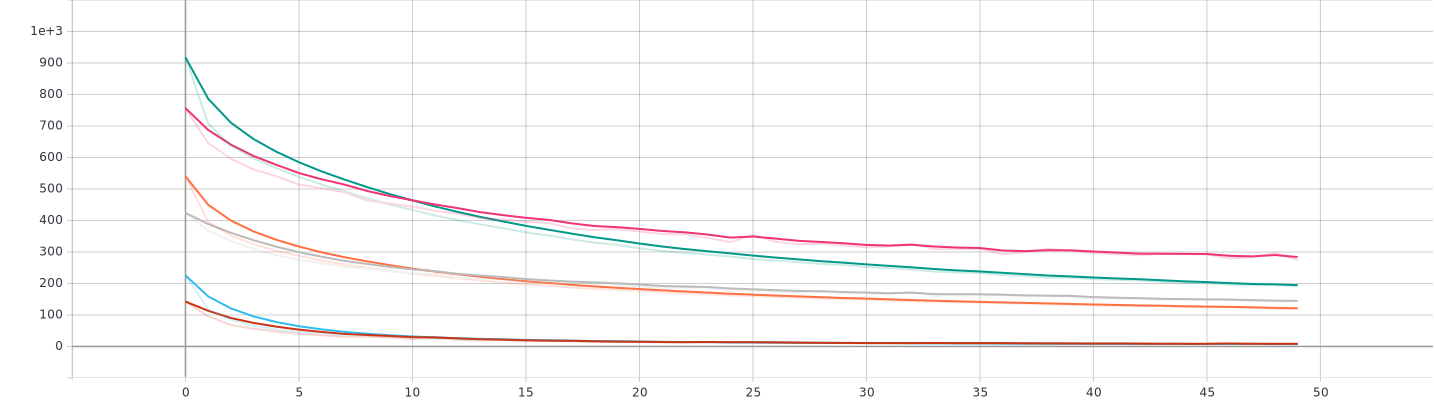
\includegraphics[width=\linewidth]{kapitel5/images//single-loss/Loss-single-loss.png}
	\caption{MSE mit 2D-Posenschätzung}
	\label{2d-poses-mse}
\end{figure}

\begin{figure}[H]
	\centering
	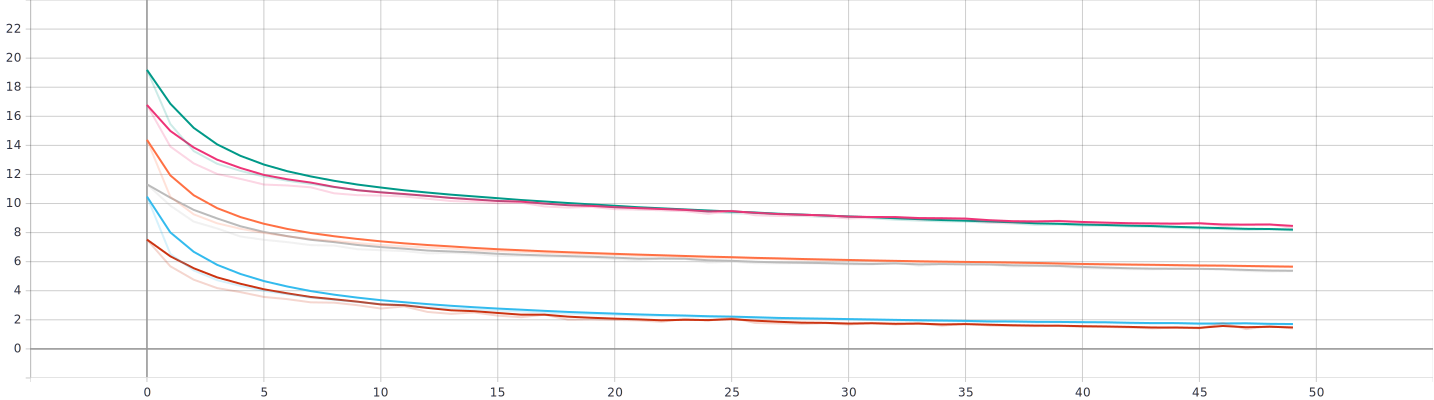
\includegraphics[width=\linewidth]{kapitel5/images/single-loss/Mean_Abs_Error_d-single-loss.png}
	\caption{MAE der Distanz mit 2D-Posenschätzung}
	\label{2d-poses-mae-d}
\end{figure}

\begin{figure}[H]
	\centering
	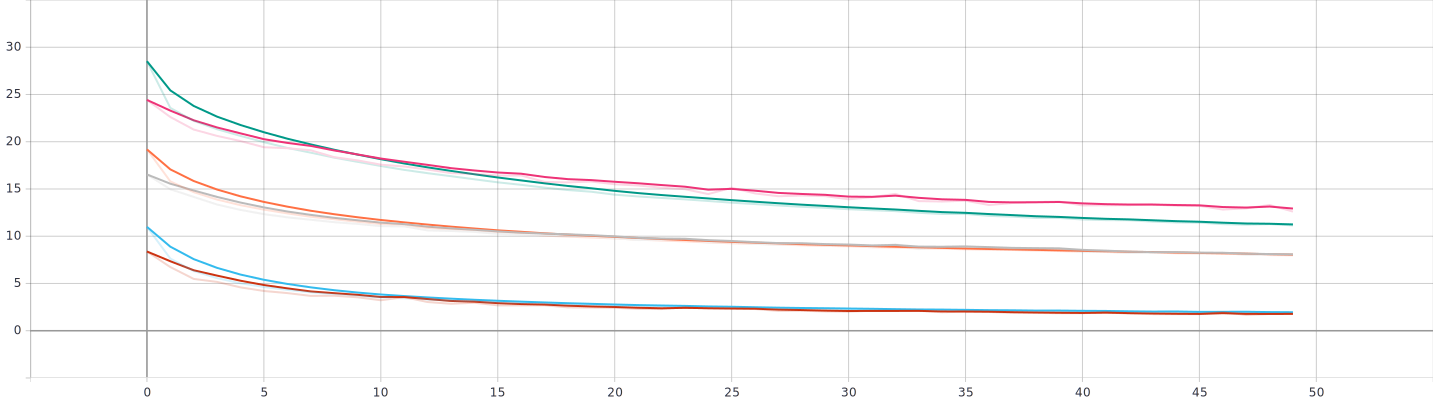
\includegraphics[width=\linewidth]{kapitel5/images/single-loss/Mean_Abs_Error_a-single-loss.png}
	\caption{MAE des Winkels mit 2D-Posenschätzung}
	\label{2d-poses-mae-a}
\end{figure}

\subsection{1D-Pose}

Das Entfernen des Winkels aus dem Zustandsvektor bringt eine leichte Verbesserung der Performance auf allen Datensätzen mit sich (siehe \ref{1d-pose-performance} und \ref{2d-pose-performance}). 

\begin{figure}[H]
	\centering
	\begin{tabular}[t]{|l|r|r|}
		\hline
		Datensatz & MSE & MAE $d$ \\
		\hline
		PD & 3.423 & 1.104 \\
		\hline
		PD-Rand & 115.4 & 6.73 \\
		\hline
		PD + PD-Rand & 60.0 & 4.364 \\
		\hline
	\end{tabular}
	\caption{Performance der 1D-Posenschätzung auf Testdaten}
	\label{1d-pose-performance}
\end{figure}

\begin{figure}[H]
	\centering
	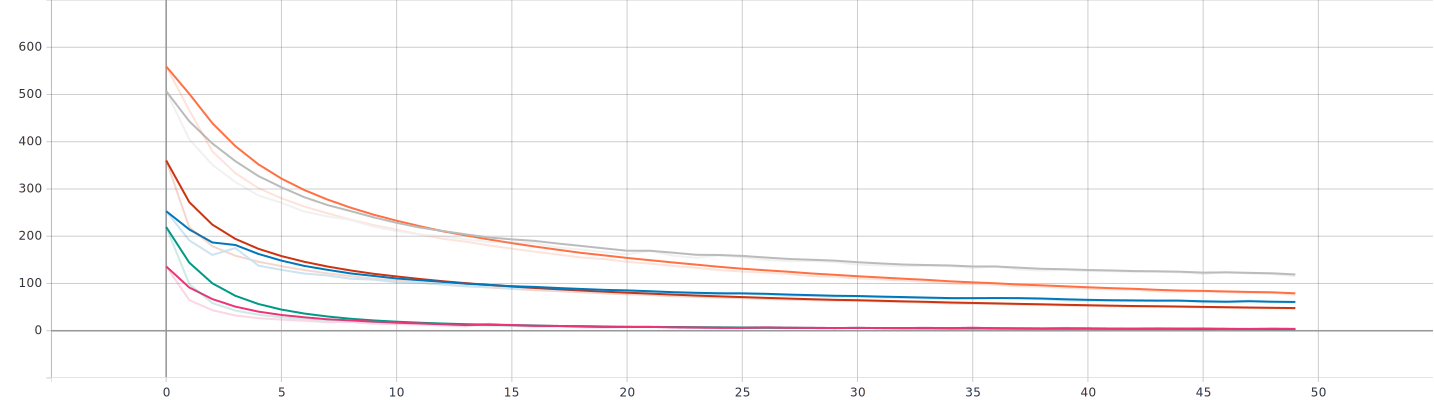
\includegraphics[width=\linewidth]{kapitel5/images/d-only/Loss-d-only.png}
	\caption{MSE der Distanz mit 1D-Posenschätzung}
	\label{1d-poses-mse-d}
\end{figure}

Allerdings führt die Reduktion auf das Schätzen des Distanzwertes allein zu einer stärkeren Überstimmung des Netzes. In \ref{1d-poses-mse-d} ist erkennbar, dass sowohl bei dem Training mit dem ``PD-Rand'' (hier in Orange für die Trainingsdaten und Grau für die Testdaten), als auch mit dem ``PD + PD-Rand'' Datensatz (Rot für Training und Blau für Test), das Netz spätestens ab Epoche 15 überstimmt ist.

\subsection{Steuerbefehl durch Expertensystem}

% \begin{figure}[H]
% 	\centering
% 	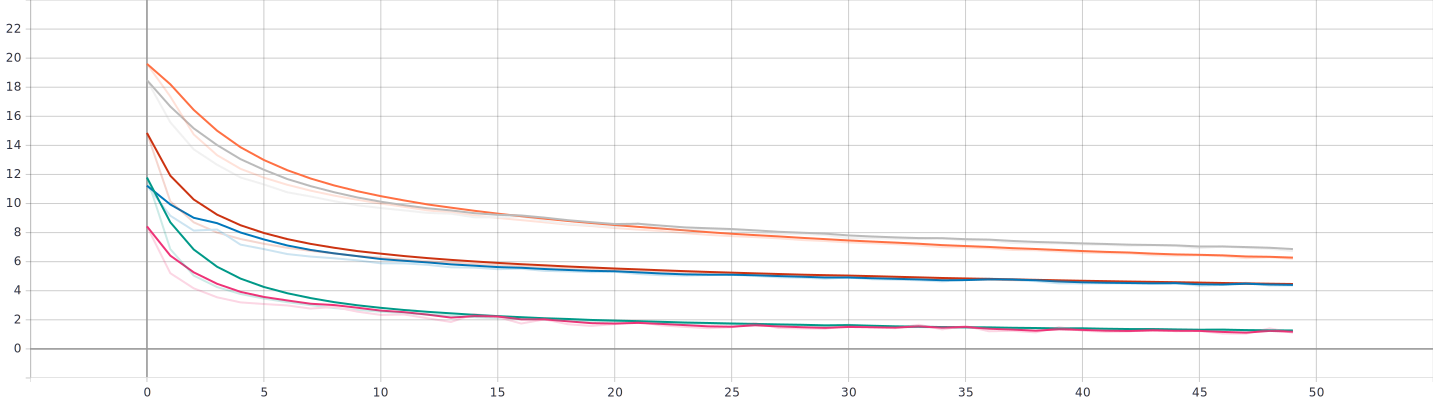
\includegraphics[width=\linewidth]{kapitel5/images/d-only/Mean_Abs_Error_d-d-only.png}
% 	\caption{MAE der Distanz mit 1D-Posenschätzung}
% 	\label{1d-poses-mae-d}
% \end{figure}

Wie zuvor zeigt sich auch hier, dass das Training mit hohem Anteil an Zufallsposen in den Daten zu einer Überstimmung des Netzes führt. So bilden sich deutliche Lücken zwischen der Performance auf Trainings- und Testdaten auf den Datensätzen ``Expert-Rand'' (Test Grau und Training Orange) und ``Expert + Expert-Rand'' (Test Blau und Training Rot) in \ref{expert-mse-omega}.


\begin{figure}[H]
	\centering
	\begin{tabular}[t]{|l|r|r|}
		\hline
		Datensatz & MSE & MAE $\omega$ \\
		\hline
		Expert & 0.00536 & 0.04214 \\
		\hline
		Expert-Rand & 0.11 & 0.205 \\
		\hline
		Expert + Expert-Rand & 0.057 & 0.1322 \\
		\hline
	\end{tabular}
	\caption{Performance der Schätzung eines Steuerbefehls auf Testdaten}
	\label{expert-performance}
\end{figure}

\begin{figure}[H]
	\centering
	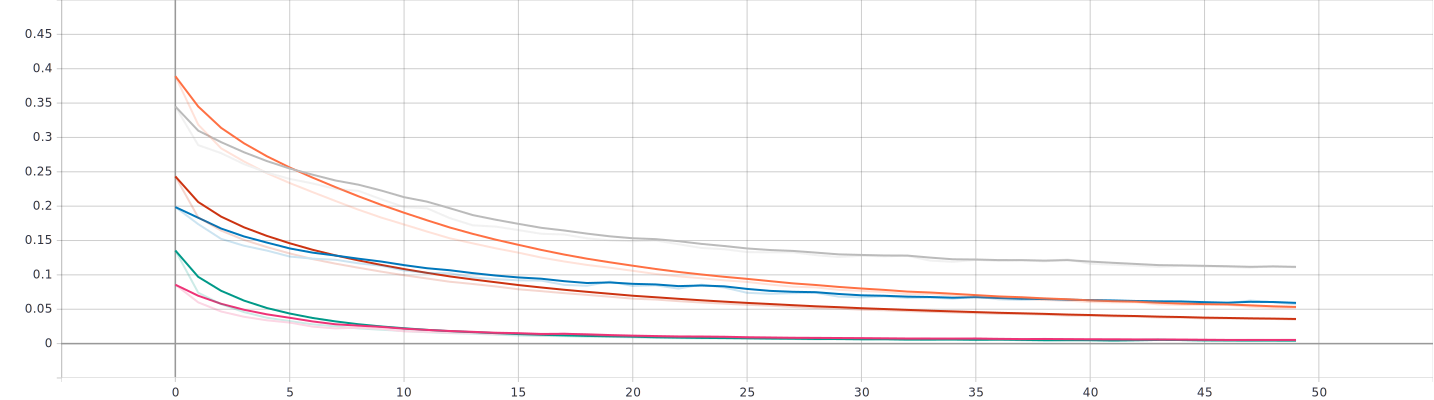
\includegraphics[width=\linewidth]{kapitel5/images/expert/Loss-expert.png}
	\caption{MSE der Winkelgeschwindigkeit mit Expertenbefehl}
	\label{expert-mse-omega}
\end{figure}

% \begin{figure}[H]
% 	\centering
% 	\includegraphics[width=\linewidth]{kapitel5/images/expert/Mean_Abs_Error_omega-expert.png}
% 	\caption{MAE der Winkelgeschwindigkeit mit Expertenbefehl}
% 	\label{expert-mae-omega}
% \end{figure}

\begin{tabular}[t]{|c|l|r|r|}
	\hline
	 & \textbf{Kacheltyp} & \textbf{MAE} & \textbf{n} \\
	\hline
	\multirow{4}{*}{PD} 
	& Alle
	& 12.59, 20.41
	& 100000\\
	\cline{2-4}
	& Gerade
	&  9.76, 13.79
	& 53433\\
	\cline{2-4}
	& Linkskurve
	& 16.70,  35.28
	& 20311\\
	\cline{2-4}
	& Rechtskurve
	& 23.78, 37.95 
	& 4728\\
	\cline{2-4}
	& 3-Wege
	&  13.27, 18.95
	& 21528\\
	\hline
	\multirow{4}{*}{PD-Rand} 
	& Alle
	& 11.63, 17.19
	& 100000\\
	\cline{2-4}
	& Gerade
	&  9.67, 13.08
	& 55325\\
	\cline{2-4}
	& Linkskurve
	& 14.38, 26.80
	& 18513\\
	\cline{2-4}
	& Rechtskurve
	& 16.44, 31.53
	& 3796\\
	\cline{2-4}
	& 3-Wege
	& 13.36, 16.97
	& 22366\\
	\hline
	\multirow{4}{*}{PD-Concat} 
	& Alle
	& 10.62, 16.37
	& 100000\\
	\cline{2-4}
	& Gerade
	& 7.67, 11.04
	& 49792\\
	\cline{2-4}
	& Linkskurve
	& 13.73, 23.53
	& 24695\\
	\cline{2-4}
	& Rechtskurve
	& 17.59, 29.68
	& 5163\\
	\cline{2-4}
	& 3-Wege
	& 12.28, 17.35
	& 20350\\
	\hline
\end{tabular}